\begin{wrapfigure}{r}{0.50\textwidth}
  \centering
  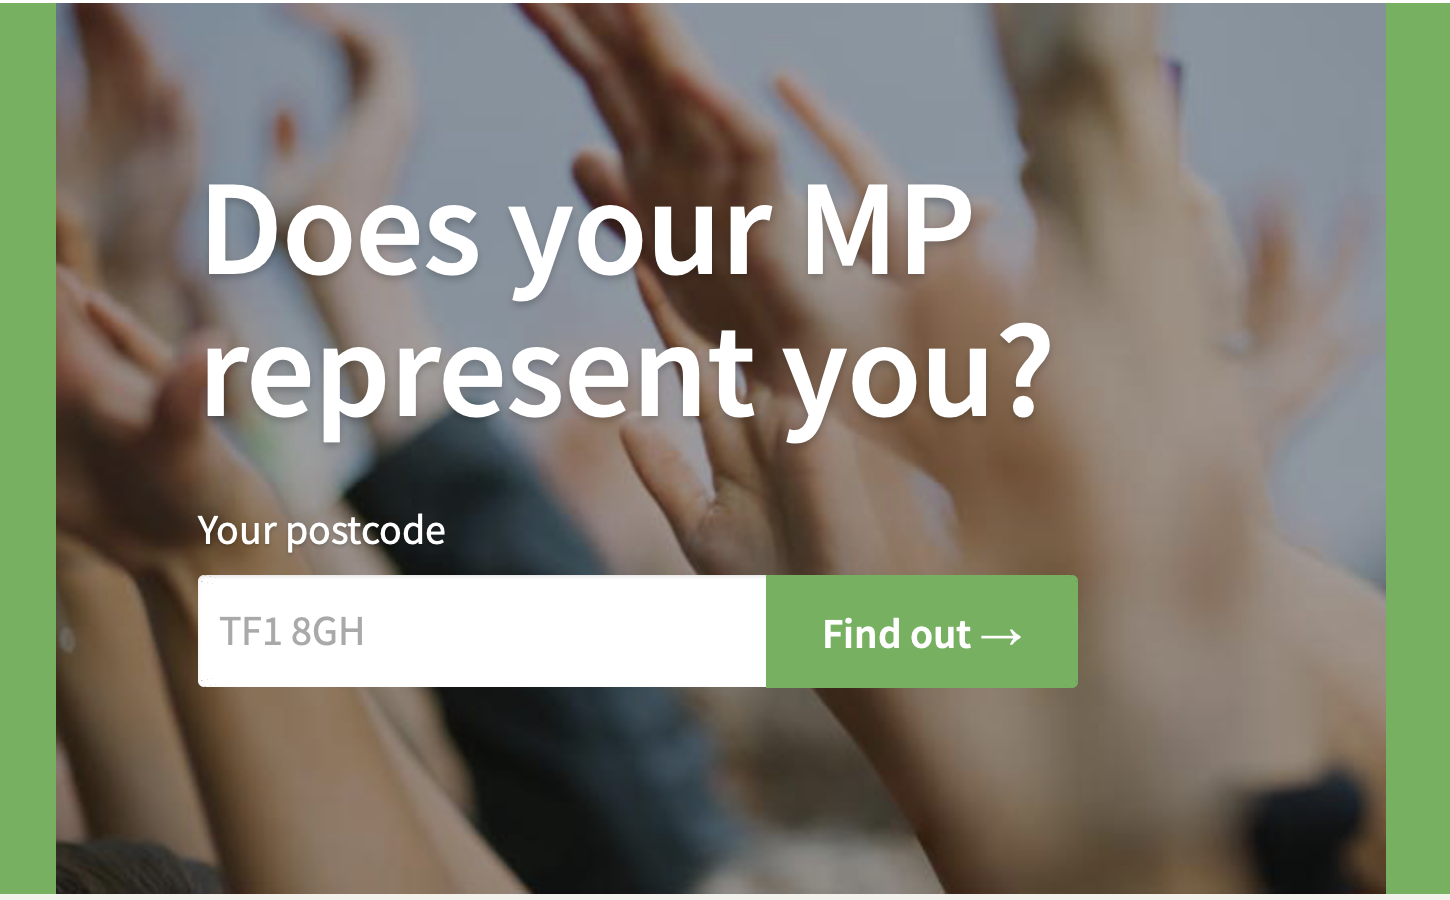
\includegraphics[scale=0.20]{images/they-work-for-you-implementation-search-box}
  \caption{Search box}
  \label{fig:they-work-for-you-implementation-search-box}
\end{wrapfigure}

The screen shot within Figure \ref{fig:they-work-for-you-implementation-search-box} depicts the home page of the site,
and prominently displayed within the home page is a search box, which, amongt other types of entries, accepts postcode \cite{postcodes-uk} values.
When a user enters a postcode within the search box the site will subsequently display information about the MP associated with the entered post code.
This clear and simple process is a good example of how the design of the site engenders accessibility,
particularly for those users who do not know the name of their MP.